\chapter{Problem Definition}
\label{chap:problem}

\section{Array Signal Processing}
\label{sec:problem_array}
In general array signal processing is concerned with three tasks: detection of noise signals, estimation of the direction of arrival and beamforming. The locations of the microphones and speakers in the room are usually stationary. These locations hold valuable information which can be used when processing the audio signal. An elaborate method to process this signal is beamforming \cite{lui2010}. This is a statistical method to estimate parameters, which is further complicated by the spatial dimensions of the array. Krim and Viberg formulate the problem of sensor array processing as: \textit{"\dots the estimation of parameters by fusing temporal and spatial information, captured via sampling a wavefield with a set of judiciously placed antenna sensors."} \cite{krim1996}.

\section{Ad-hoc}
\label{sec:problem_ad-hoc}
The techniques used in beamforming are not strictly valid for microphone sensor arrays, but may also hold for other types of sensor arrays. The geometry, size and number of the sensor array can vary. The geometry of the sensor array may vary from linear, circular or spherical to arbitrary geometries. This research focuses on the last type of geometry, which we will call an \textit{ad-hoc microphone array}.

\section{Near-field}
\label{sec:problem_near-field}
There is an important distinction to be made with respect to the dimensions of the array or \textit{aperture} size. There exist different methods for \textit{far-field} and \textit{near-field} beamforming. In far-field one can assume that the wave field originates from a distance far greater than the dimensions of the array, which leads to the assumption that the wave field has a flat wave front. This means that the Direction Of Arrival (DOA) is the same for every sensor in the array. In near-field beamforming the distance from the source of the wave field to the array is comparable in magnitude to the dimensions of the array. This means that every sensor gets a different DOA and amplitude of the signal. \newline
An often used rule to decide whether the far-field approximation is valid is $r = 2L^2/\lambda$ where $r$ the distance from the microphone array to the source, $L$ the largest array dimension and $\lambda$ the operating wavelength \cite{kennedy1998}. In the scenario outlined in section {\ref{chap:introduction}} the dimensions of the microphone array are large with respect to the distance between the array and the source. Therefore, according to the earlier mentioned rule, we can assume that the sources of interest are in the near-field region \cite{gaubitch2014}. In addition, the positioning of the microphones is arbitrary, but known. As such, the main focus for our implementation will be near-field beamforming with ad-hoc microphone arrays. 

\nomenclature{$L$}{Largest array dimension [m]}
\nomenclature{$\lambda$}{Wavelength [m]}

\section{Broadband}
\label{sec:problem_broadband}
There is one more distinction to be made in type of the beamformer. There are different design techniques for broadband and narrowband beamformers. In speech communication applications broadband design implies design over several octaves. In order to use the processed signals for speech communications, the beamformers have to perform well over the frequency band from $300 Hz$ to $3400 Hz$ \cite{ituspeechfreq2011}.

\section{Observation Model}
\label{sec:observation}

Figure \ref{fig:observation} shows a representation of a room with some $x$, $y$ and $z$ dimensions and $M$ microphones. An acoustic source signal $s(t)$ originating from a position $\textbf{p}_{src}^{j}$ will propagate through the room and reach all the microphones positioned at $\textbf{p}_{mic}^{i}$. At a time $t$ the sampled microphone signal for each microphone consists of delayed and attenuated versions of the source signal $a_{i}s(t-\tau_{i})$ with undesired signal components $v_{i}(t)$ added to it. The acoustic transfer function (ATF) of the room is denoted by $h_{i}(t)$. For this research the ATF of an anechoic room is assumed unless otherwise specified:

\nomenclature{$M$}{Number of microphones}
\nomenclature{$\textbf{p}$}{Position vector in space [m]}
\nomenclature{$t$}{Time [s]}
\nomenclature{$s(t)$}{Acoustic source signal in the time domain}
\nomenclature{$a$}{Attenuation coefficient [$\text{m}^{-1}$]}
\nomenclature{$\tau$}{Delay of a signal [s]}
\nomenclature{$v(t)$}{Undesired signal components in the time domain}
\nomenclature{$h(t)$}{Acoustic transfer function in the time domain}

\begin{equation}
\label{eq:ATF}
H_{i,j}(\omega) = \frac{\exp(-j\omega \dfrac{r_{i,j}}{c})}{4\pi r_{i,j}}
\end{equation}

\nomenclature{$H(\omega)$}{Acoustic transfer function in the frequency domain}
\nomenclature{$r$}{Distance between source and mic [m]}
\nomenclature{$c$}{Speed of sound [m/s]}

with
\begin{equation}
r_{i,j} = \norm{\textbf{p}_{mic}^{i}-\textbf{p}_{src}^{j}}
\end{equation}

where $c$ is the speed of sound; $\textbf{p}$ is the position vector in space. In many cases there will be only one source of interest, so the $j$ index may be omitted.
The ATF is represented in the Fourier domain. The positions and orientations of the microphones and sources are assumed to be known. The ATF describes the set of all the propagation paths from a source to a microphone and hence the convolution between the sound coming from the source and the impulse response results in the sound recorded by the microphones. If the microphone has nonuniform directivity gain the room ATF is convolved over time with the directivity pattern of the microphone $g(t,\theta,\phi)$:

\begin{equation}
\label{eq:look}
d_{i}(t,\theta,\phi) = h_i(t) \ast g_i(t,\theta,\phi)
\end{equation}

\nomenclature{$d(t,\theta,\phi)$}{Array response vector [s]}
\nomenclature{$g(t,\theta,\phi)$}{Directivity pattern of a microphone in the time domain}
\nomenclature{$\theta$}{Azimuth [$\degree$]}
\nomenclature{$\phi$}{Elevation [$\degree$]}

where "$\ast$" denotes the convolution; $g_i(t,\theta,\phi)$ is the directivity impulse response \cite{BAP:RosalieTim} of the specific microphone, $\theta$ and $\phi$ are the azimuth and elevation angles between the source and the respective microphone. This directivity pattern was measured in the anechoic chamber of the Faculty of Applied Sciences at TU Delft for the smartphones used in this research. For omnidirectional microphones a Kronecker delta can be used for $g_i$, or it can simply be omitted. We can combine the attenuation and delay for all microphones into one vector:

\begin{equation}
\textbf{d}(\omega,\theta,\phi) = [A_{1}(\omega,\theta,\phi)e^{-j\omega\tau_{1}},A_{2}(\omega,\theta,\phi)e^{-j\omega\tau_{2}},...,A_{M}(\omega,\theta,\phi)e^{-j\omega\tau_{M}}]^{T}
\end{equation}

\nomenclature{$\textbf{d}(\omega,\theta,\phi)$}{Look vector of the array}
\nomenclature{$y(t)$}{Received audio signal by a microphone in the time domain}

where $\textbf{a}^{T}$ denotes the transpose of the vector $\textbf{a}$. The vector $\textbf{d}$ is called the \textit{look vector} of the array. $A_{i}$ is the combined attenuation factor due to the ATF and the directivity $\tau_{i}$ is the combined delay due to the ATF and the directivity.
\\
We model the received signals ${y}_{i}(t),i \in \left\{ {1,...,M}\right\}$ at each sensor using equation \ref{eq:look} as:

\begin{equation}
\label{eq:observationtime}
{y}_{i}(t) = a_{i}s(t-\tau_{i}) \ast g_i(t,\theta,\phi) + v_i(t)
\end{equation}

where $v_i(t)$ denotes the undesired signal components which consist of noise and reverberations (the dotted lines in figure \ref{fig:observation}) and signals from interfering sources. $a_i$ is the attenuation factor due to the ATF. The delay between when the signal is at the reference microphone and the $i^{th}$ microphone is $\tau_{i} = \norm{\textbf{p}_{mic}^{i}-\textbf{p}_{src}}/c$ where $c$ denotes the speed of sound.

\begin{figure}[h!]
	\centering  
	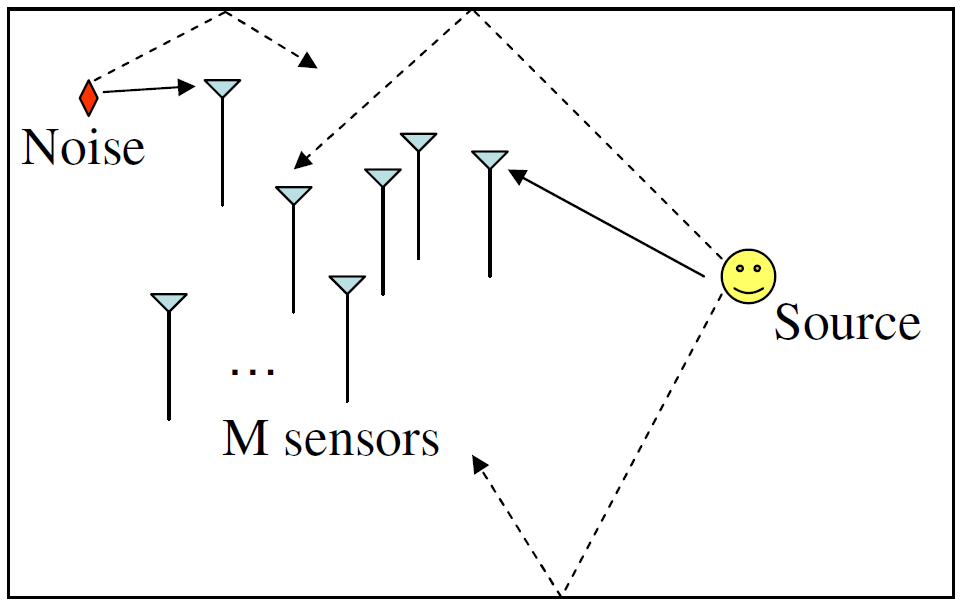
\includegraphics[scale=0.7]{observation_model.png}
	\caption[Room representation for the observational model \cite{ba2007}]{A source incident on an array of M sensors in the presence of noise and reverberations \cite{ba2007}}
	\label{fig:observation}
\end{figure}

In the Fourier domain the received signal described in equation \ref{eq:observationtime} for microphone $i$ can be written as:
\begin{equation}
\label{eq:observationfreq}
Y_{i}(\omega) = A_{i}(\omega)S(\omega)e^{-j\omega\tau_{i}} G_i(\omega,\theta,\phi) + V_{i}(\omega)
\end{equation}

\nomenclature{$Y(\omega)$}{Received audio signal by a microphone in the frequency domain}
\nomenclature{$A(\omega,\theta,\phi)$}{Attenuation coefficient in the frequency domain, as a function of the look direction}
\nomenclature{$S(\omega)$}{Source signal in the frequency domain}
\nomenclature{$G(\omega,\theta,\phi)$}{Directivity pattern of a microphone in the frequency domain}
\nomenclature{$V(\omega)$}{Undesired signal components in the frequency domain}


The attenuation factor $A_{i}(\omega)$ can depend on the frequency. $G_i(\omega,\theta,\phi)$ is the directivity pattern of the microphone in the Fourier domain, for nonuniform directivity microphones on the respective azimuth and elevation; $V_{i}(\omega)$ is the additive noise in the Fourier domain.

By choosing the values for $A_{i}(\omega,\theta,\phi)$ and $\tau_{i}$ one can maximize the gain (or steer the beam) in any direction spanned by the position vectors of the array. The desired signal can be recovered by multiplying the microphone signals by a complex weighing factor $\textbf{w}$:

\begin{equation}
\label{eq:bf_est}
\hat{S}(\omega) = \textbf{w}^{H}(\omega)\textbf{Y}(\omega)
\end{equation}

\nomenclature{$\hat{S}(\omega)$}{Estimated source signal}
\nomenclature{$\textbf{w}(\omega)$}{Vector of complex weighing factors}

where $\textbf{a}^{H}$ denotes the Hermitian transpose of the vector $\textbf{a}$. The estimated signal $\hat{S}(\omega)$ can finally be transferred back to the time domain to arrive at the beamformed audio signal. Sections \ref{sec:des_dsb} and \ref{sec:des_mvdr} go into how to calculate the weights $\textbf{w}(\omega)$.
